\section{Solution}
\label{Solution}
%In the solution section, the answers to the research questions or the solutions from the research hypotheses are presented in detail. The relation to the research questions or the research hypotheses should explicitly (by using their names) be given. I.e. this section answered the question ”What is the solution?”. First of all, the necessary formalisms are defined. Please note that a compromise between a clear, formalized presentation and textual explanations should be found. Normally each community has a more or less standardized formalism which should be re-used. Next, the main idea, i.e. the gist of the solution approach is defined. Often figures help to convey the main solution idea. Finally, the solution is presented in detail. Often, formal algorithm definitions or mathematical methods are defined. Please note that all steps of algorithms or solution methods must also be explained textually. This section must be self-contained and allow for a re-implementation of the solution by the reader.

\begin{figure*}[ht]
\centering
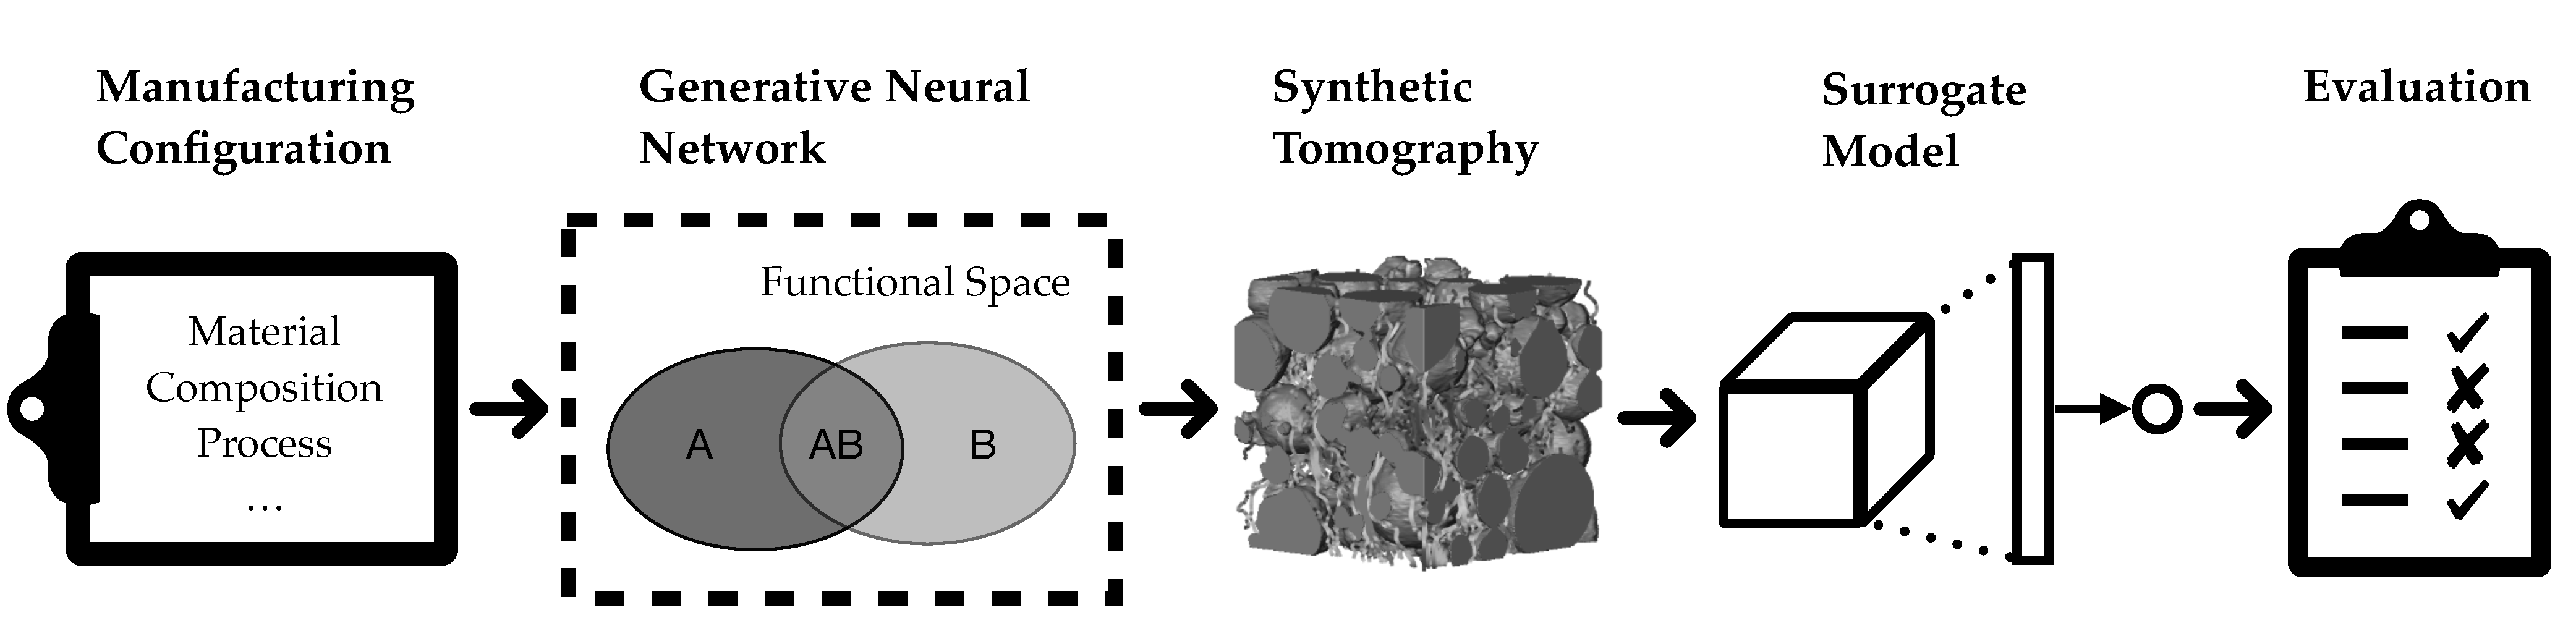
\includegraphics[width=\textwidth]{images/Morph.pdf}
\caption{Closed framework for morphological system description. A generative neural network synthesizes possible tomographies (CTs) of material composites or assemblies based on predefined manufacturing configurations. The morphological representation enables the visualization of various manufacturing influences. A surrogate model is based on the spatial representation and describes the physical properties. This finally enables an evaluation of the materials design}
\label{fig:Framework}
\end{figure*}
ML, CT, and experiments are combined here, to automatically construct transferable and interpretable constitutive materials laws, which are currently missing for the design of many complex material composites. As a result, a new method is developed to learn surrogate models for materials and assemblies. 

\subsection{Surrogate Design Model}
\label{Surrogate_Model}
A bottleneck in traditional materials design is the time consuming design-test-cycle: Each new material has to be designed, produced and then experimentally tested. Direct simulation is only a partial solution, as both modeling and simulation tasks are time-consuming, require a high level of expertise and significant computational resources to solve even small domains. A solution for the problem is a machine learning surrogate model which is a simplified and computationally less expensive model that serves as a substitute for time-consuming simulations or expensive computations.

Based on bulk materials data, a model generation function can be learned that maps new materials designs onto materials models. Such predictions can be used to try other, new materials designs. Maybe better: Even if this neural network-based approach yields less quantitative precision for a single material. Unbiased learning of a predictive model can still be expected to be qualitatively more predictive than traditional ad hoc heuristics.

Such an approach is sketched in Figure~\ref{fig:workflow}: 
The strategy is three-fold. A targeted experimental program generates a range of materials from which CTs are synthesized to create a data set of typical morphologies. The synthesised materials are then tested for their properties to generate a validation dataset ${\cal E}$, while the CTs are feed into the second layer of physical modelling. The main purpose of this layer is to efficiently expand the training set by overlaying the morphologies with available bulk properties to simulate the behavior of a much larger set of materials. This wouldn't be possible experimentally. The layer thoroughly maps the relationship between bulk properties and morphologies. These are expressed by feature vectors build from materials properties (e.g., porosity $\epsilon_p$, tortuosity $\tau$, strut lengths $l$ etc.)  It also implements a map $p({\bf r})\rightarrow \left\{\epsilon_p,\tau,...\right\}$ through image-processing techniques, which encodes CTs into feature vectors. This large-scale dataset underpins the training phase. Based on this data -- augmented with and validated against real experiments -- a neural network is trained. Later during the operation phase, new materials designs -- expressed by the feature vectors and materials properties -- become input to this network which then predicts the probable corresponding materials model. 

\subsection{Algorithmic Representation}
\label{Algortith_Repr}
Because these materials models come in form of a neural network, explainability and traceability become challenges. For this reason, explicit, formula-based models are extracted from the neural network. Such models resemble closely current manual materials models but can qualitatively differ as a function of provided feature vectors. However, to prevent neural networks from remaining black boxes, changes to the network topology and learning process are required. For this (see also Figure \ref{fig:workflow}) a surrogate model in form of a neural network is learned. This model replaces the previous physical simulations but has the advantage of predicting the materials behavior very quickly. Using such a surrogate model has several advantages: (i) Its topology can be optimized towards the symbolic formula extraction, e.g. by disentanglement of latent variables (RepL). (ii) By using Bayesian principles of uncertainty estimation, the surrogate model can actively ask for more data points when needed. (iii) The surrogate model can be created in a way which supports inter- and extrapolation -- mainly by adding physical information to the network topology and the priors on latent variables. Finally, symbolic formula extraction algorithms and algorithms from the field of explainable AI are used to extract symbolic formulas. These learned formulas guide the design process, e.g. by helping to identify optimal materials designs for specific tasks or identifying promising candidates for targeted experiments.

\subsection{Morphological Representation}
\label{Morph_Repr}
Due to a symbolic description, the physical materials behavior can be theoretically interpreted. However, the generated equations are often difficult to interpret in practice due to their complexity. Another way to better understand system relationships is to synthesize materials structures in the form of tomography. This approach is visualized in Figure \ref{fig:Framework}.

The generative part uses CTs as training data. These are labeled with manufacturing configurations such as material compositions and process parameters. Under these high-dimensional conditions, a GAN or DDPM is trained to synthesize high-resolution 3D tomography data. In the operation phase, the respective influence on the morphological structure is analyzed by varying the conditions. Analogous to the unsupervised approach mentioned above, a surrogate model is then used to learn and represent the materials behavior. Finally, the design draft is evaluated.